\documentclass[mathserif,11pt]{beamer}

\usepackage{url,verbatim,natbib}
\usepackage[english]{babel}
\usepackage{amsmath, mathabx}
\usepackage{dsfont}
\usepackage[headheight=22pt]{beamerthemeboxes}
\usepackage{graphicx}
\beamertemplatenavigationsymbolsempty 
\setbeamercovered{transparent}

\setbeamertemplate{itemize item}{$\bullet$} 
\setbeamercolor{title}{fg=uio}
\setbeamertemplate{sections/subsections in toc}[ball unnumbered]
\setbeamercolor{section in toc}{fg=uio,bg=white}
\setbeamercolor{subsection in toc}{fg=uio,bg=white}
\setbeamercolor{result}{fg=black, bg=yellow}
\newcommand{\dotsim}{\stackrel{\cdot}{\sim}}
\newcommand{\interi}{{\rm Z}\negthinspace\negthinspace {\rm Z}}
\newcommand{\reali}{{\rm I}\negthinspace {\rm R}}
\newcommand{\naturali}{{\rm I}\negthinspace {\rm N}}
\newcommand{\sign}{\mathop{\rm sgn}\nolimits}
\newcommand{\sgn}{\mathop{\mathrm{sgn}}}
\definecolor{redve}{rgb}{0.604,0.008,0.00}
\definecolor{lmu}{rgb}{0.188,0.522,0.306}
\definecolor{uio}{rgb}{0.847,0.118,0.02}

\def\R{{\rm I\!R}}
\def\P{{\rm Pr}}
\def\Real{{\rm I\!R}}
\def\T{{\footnotesize {^{_{\sf T}}}}}
\def\tr{{\rm tr}}
\def\diag{{\rm diag}}


\useframetitletemplate{% 
\begin{centering} 
\begin{small} \structure{\textcolor{uio} \insertframetitle {\insertframesubtitle}}
\end{small}

\end{centering} 
}

\addheadboxtemplate{\color[rgb]{1,1,1}}{\color{uio} \underline{{\hspace{5pt}\includegraphics[scale=0.06]{../../../../support/uio_logo_eng} \hspace{0.265\paperwidth}\color{black} \tiny  STK-IN4300 - Statistical Learning Methods in Data Science} \hspace{5pt}}}

%\bfseries{\insertsection}

\addfootboxtemplate{\color[rgb]{1,1,1}}{\color{black} \tiny \quad  
STK4030: lecture 1
  \hfill \tiny \insertframenumber / \inserttotalframenumber \hspace{5pt}}

  
\title{STK-IN4300 \\ Statistical Learning Methods in Data Science}
\author{Riccardo De Bin} 
\institute{debin@math.uio.no} 
\date{}


\begin{document}
\setbeamercolor{bgr}{fg=black,bg=uio}

{
\setbeamertemplate{headline}{}
\frame{
\vspace{-2cm}
\begin{beamercolorbox}[sep=-2.2em,wd=5cm,colsep=0.5pt,ht=4.25ex,dp=3ex,left]{postit}
\includegraphics[scale=0.06]{../../../../support/uio_logo_eng}
\end{beamercolorbox}
\vspace{0.365cm}
\noindent\makebox[\linewidth]{\color{uio} \rule{\paperwidth}{0.4pt}}
\vspace{2.5cm}
\titlepage
}
}

\frame{\frametitle{Outline of the lecture}
\tableofcontents
}


%%%%%%%%%%%%
\section{Introduction}
%%%%%%%%%%%%

\frame{\frametitle{Introduction: }
\framesubtitle{Elements of Statistical Learning}
\begin{columns}
\begin{column}{0.65\textwidth}
This course is based on the book:\\ \textcolor{uio}{``The Elements of Statistical Learning: Data Mining, Inference, and Prediction''} \\ by T. Hastie, R. Tibshirani and J. Friedman:
\begin{itemize}
  \item reference book on modern statistical methods;
  \item free online version, \url{https://web.stanford.edu/~hastie/ElemStatLearn/}.
\end{itemize}
\end{column}
\begin{column}{0.35\textwidth}
 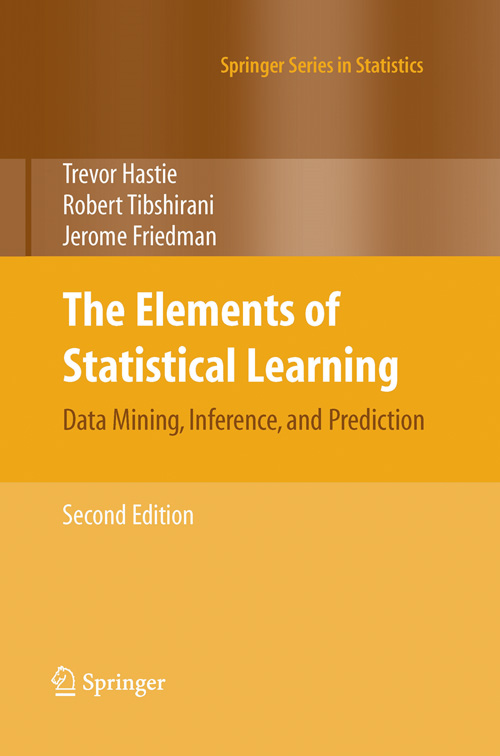
\includegraphics[width=\textwidth]{Cover.jpg}
\end{column}
\end{columns}
}


\frame{\frametitle{Introduction: }
\framesubtitle{statistical learning}
\begin{center}
\it ``We are drowning in information, but we starved from knowledge'' (J. Naisbitt)
\end{center}
\begin{itemize}
\item nowadays a \textcolor{uio}{huge quantity of data} is continuously collected \\ $\Rightarrow$ a lot of \textcolor{uio}{information} is available;
\item we struggle with profitably using it;
\end{itemize}

\vspace{1cm}

The \textcolor{uio}{goal of statistical learning} is to ``get knowledge'' from the data, so that the information can be used for prediction, identification, understanding, \dots
}


\frame{\frametitle{Introduction: }
\framesubtitle{email spam example}
Goal: construct an automatic spam detector that block spam.
Data: information on 4601 emails, in particular,
\begin{itemize}
  \item whether was it spam (\texttt{spam}) or not (\texttt{email});
  \item the relative frequencies of 57 of the most common words or punctuation marks.
\end{itemize}

\vspace{0.5cm}

\begin{tabular}{l|rrrrrrrr}
\hline
word  & george &  you & your &   hp & free &  hpl &    ! & \dots \\
\hline
spam  &   0.00 & 2.26 & 1.38 & 0.02 & 0.52 & 0.01 & 0.51 & \dots \\
email &   1.27 & 1.27 & 0.44 & 0.90 & 0.07 & 0.43 & 0.11 & \dots \\
\hline
\end{tabular}

\vspace{0.5cm}

Possible rule: if (\texttt{\%george} $<$ 0.6) \& (\texttt{\%you} $>$ 1.5) then \texttt{spam} \\
\hspace{8.1cm} else \texttt{email}
}


\frame{\frametitle{Introduction: }
\framesubtitle{prostate cancer example}
\begin{columns}
\begin{column}{0.48\textwidth}
\vspace{-0.75cm}
\begin{figure}
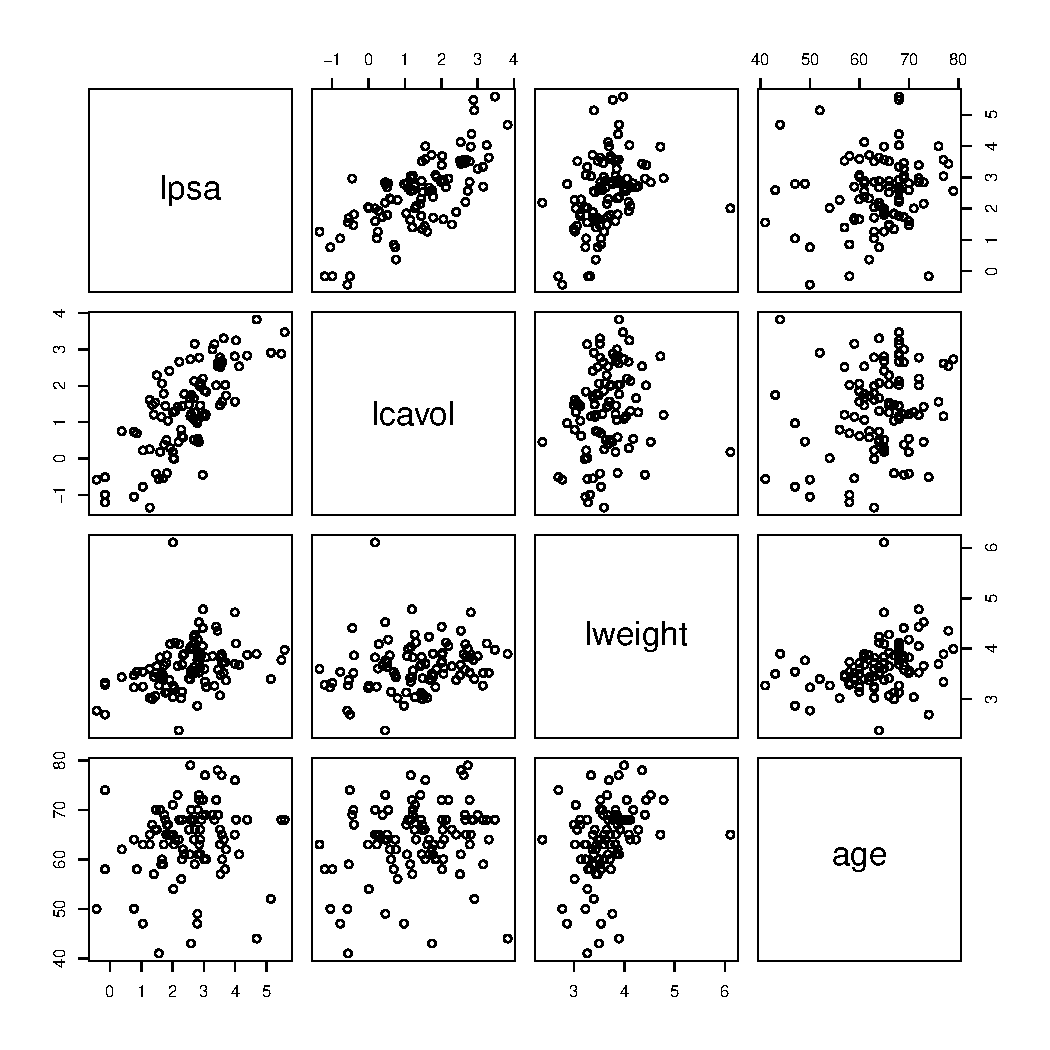
\includegraphics[width=1.25\textwidth]{prostate}
\end{figure}
\end{column}
\begin{column}{0.48\textwidth}
\begin{itemize}
  \item data from \cite{StameyAl1989};
  \item goal: predict the level of (log) prostate specific antigene (\texttt{lpsa}) from some clinical measures, such as log cancer volume (\texttt{lcavol}), log prostate weight (\texttt{lweight}), age (\texttt{age}), \dots;
  \item possible rule: $f(X)=0.32 \texttt{ lcavol} + 0.15 \texttt{ lweight} + 0.20 \texttt{ age}$ 
\end{itemize}
\end{column}
\end{columns}
}


\frame{\frametitle{Introduction: }
\framesubtitle{handwritten digit recognition}
\begin{columns}
\begin{column}{0.48\textwidth}
\vspace{-0.75cm}
\begin{figure}
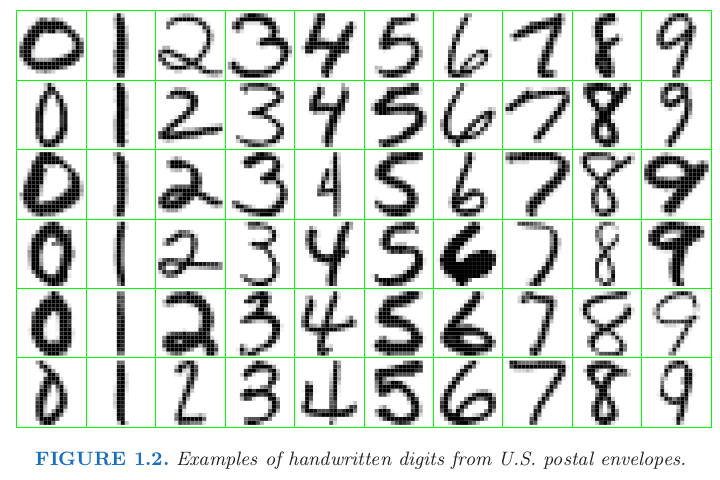
\includegraphics[width=1.2\textwidth]{digits}
\end{figure}
\end{column}
\begin{column}{0.48\textwidth}
\begin{itemize}
  \item data: 16 x 16 matrix of pixel intensities;
  \item goal: identify the correct digit (0,, \dots, 9);
  \item the outcome consists of 10 classes.
\end{itemize}
\end{column}
\end{columns}
}


\frame{\frametitle{Introduction: }
\framesubtitle{other examples}
Examples (from the book):
\begin{itemize}
\item predict whether a patient, hospitalized due to a heart attack, will have a second heart attack, based on demographic, diet and clinical measurements for that patient;
\item predict the price of a stock in 6 months from now, on the basis of company performance measures and economic data;
\item identify the numbers in a handwritten ZIP code, from a digitized image;
\item estimate the amount of glucose in the blood of a diabetic person, from the infrared absorption spectrum of that person’s blood;
\item identify the risk factors for prostate cancer, based on clinical and demographic.
\end{itemize}
}


\frame{\frametitle{Introduction: }
\framesubtitle{framework}
In a typical scenario we have:
\begin{itemize}
  \item an \textcolor{uio}{outcome} $Y$ (dependent variable, response)
  \begin{itemize}
  	\item \textcolor{uio}{quantitative} (e.g., stock price, amount of glucose, \dots);
  	\item \textcolor{uio}{categorical} (e.g., heart attack/no heart attack)
  \end{itemize}
\end{itemize}
that we want to predict based on 
\begin{itemize}
  \item a set of \textcolor{uio}{features} $X_1, X_2, \dots, X_p$ (independent variables, predictors)
  \begin{itemize}
  	\item examples: age, gender, income, \dots
  \end{itemize}
\end{itemize}

In practice,
\begin{itemize}
  \item we have a \textcolor{uio}{training set}, in which we observe the outcome and some features for a set of observations (e.g., persons);
  \item we use these data to construct a \textcolor{uio}{learner} (i.e., a rule $f(X)$), which provides a prediction of the outcome ($\hat{y}$) given specific values of the features.
\end{itemize}
}


\frame{\frametitle{Introduction: }
\framesubtitle{supervised vs unsupervised learning}
The scenario above is typical of a \textcolor{uio}{supervised learning problem}:
\begin{itemize}
  \item the \textcolor{uio}{outcome is measured in the training data}, and it can be used to construct the learner $f(X)$;
\end{itemize}
In other cases only the features are measured $\rightarrow$ \textcolor{uio}{unsupervised learning problems}:
\begin{itemize}
  \item identification of clusters, data simplification, \dots
\end{itemize}

\begin{figure}
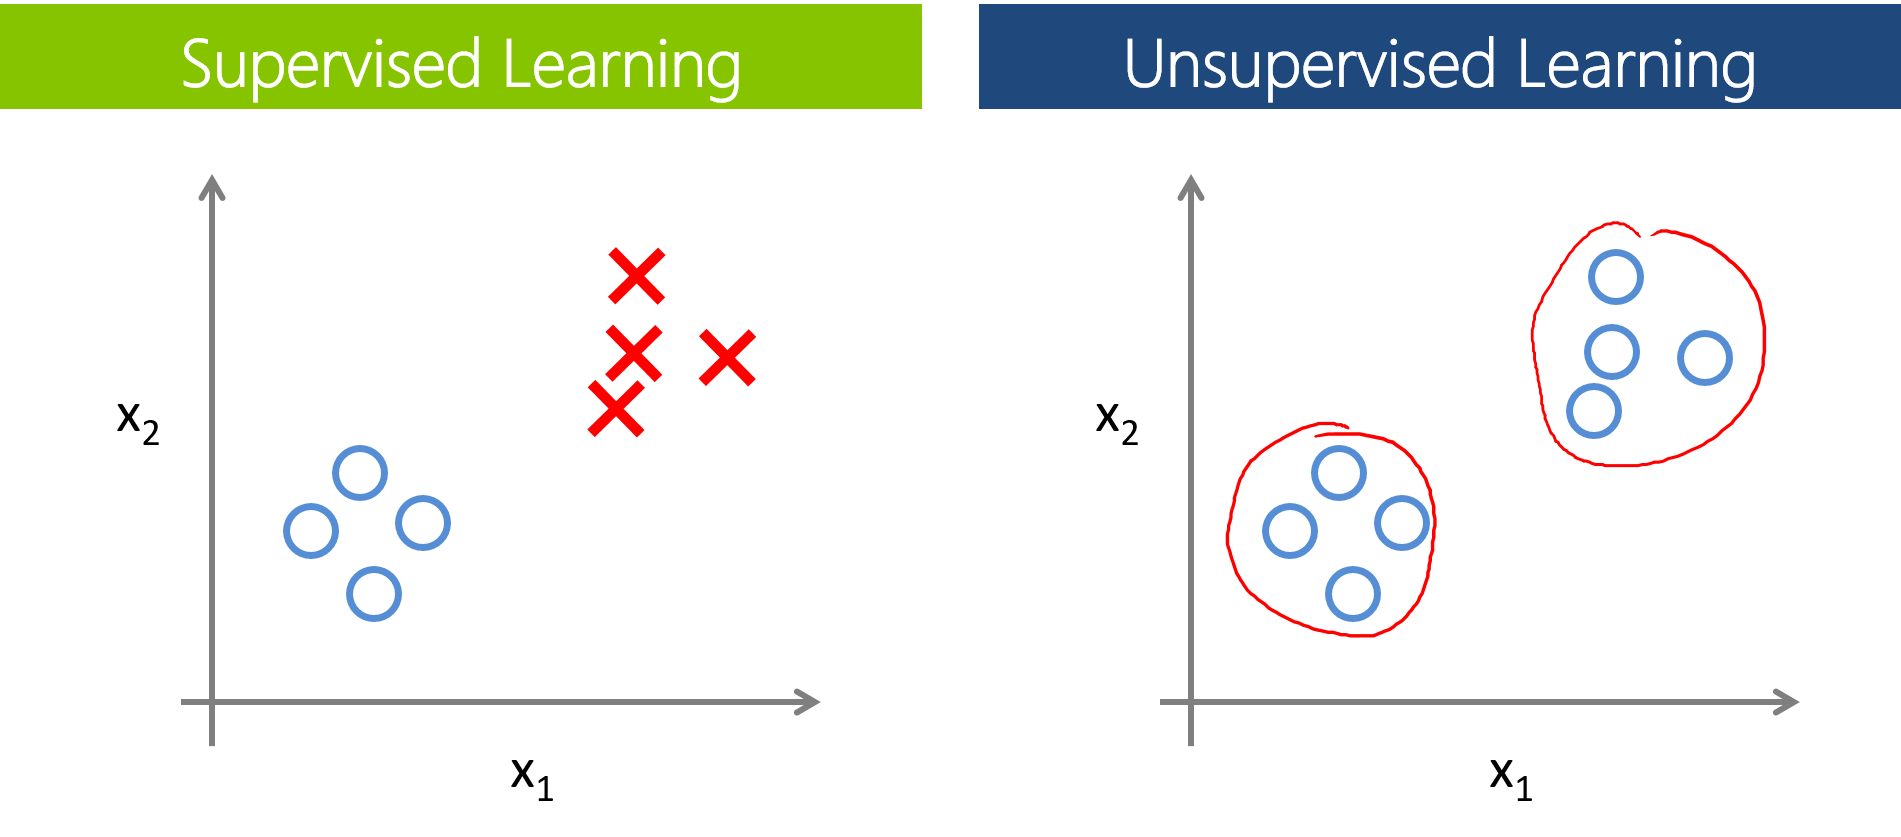
\includegraphics[width=0.95\textwidth]{supervised_unsupervised}
\end{figure}
}


\frame{\frametitle{Introduction: }
\framesubtitle{gene expression example}
\begin{columns}
\begin{column}{0.46\textwidth}
\vspace{-1cm}
\begin{figure}
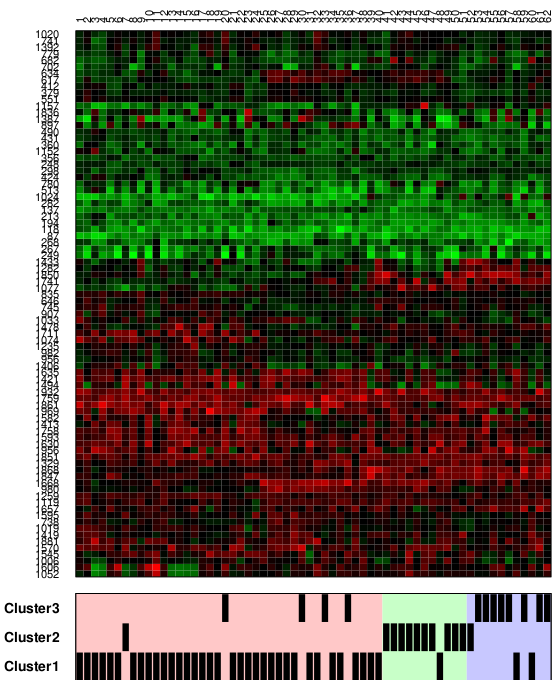
\includegraphics[width=1.2\textwidth]{heatmap}
\end{figure}
\end{column}
\begin{column}{0.54\textwidth}
\begin{itemize}
  \item heatmap from \cite{DebinRisso2011}: 62 obs vs a subset of the original 2000 genes
  \begin{itemize}
  \item \textcolor{uio}{$p>>n$ problem};
  \end{itemize}
  \item goal: group patients with similar genetic information (cluster);
  \item alternatives (if the outcome was also available):
  \begin{itemize}
  \item classify patients with similar disease (classification);
  \item predict the chance of getting a disease for a new patient (regression).
  \end{itemize}
\end{itemize}
\end{column}
\end{columns}
}


\frame{\frametitle{Introduction: }
\framesubtitle{the high dimensional issue}
Assume a training set $\{(x_{i1}, \dots, x_{ip}, y_i), i = 1,...,n\}$, where \textcolor{uio}{$n=100, p=2000$};
\begin{itemize}
  \item possible model: $y_i=\beta_0+\sum_{j=1}^p\beta_jx_{ij}+\varepsilon_i$;
  \item least squares estimate: $\hat{\beta}=(X^T X)^{-1} X^T y$.
\end{itemize}
Exercise:
\begin{itemize}
  \item go together in groups of 3-4;
  \item learn the names of the others in the group;
  \item discuss problems with the least squares estimate in this case;
  \item discuss possible ways to proceed;
\end{itemize}
}

\frame{\frametitle{Introduction: }
\framesubtitle{the high dimensional issue}
Major issue: $X^T X$ is \textcolor{uio}{not invertible}, infinitely many solutions!

\vspace{0.5cm}

Some possible directions:
\begin{itemize}
  \item \textcolor{uio}{dimension reduction} (reducing $p$ to be smaller than $n$),
  \begin{itemize}
    \item remove variables having low correlation with response;
	\item more formal subset selections;
	\item select a few ``best'' linear combinations of variables;
  \end{itemize}
  \item \textcolor{uio}{shrinkage methods} (adding constrain to $\beta$),
  \begin{itemize}
    \item ridge regression;
    \item lasso (least absolute shrinkage and selection operator)
    \item elastic net.
  \end{itemize}
\end{itemize}
}


\frame{\frametitle{Introduction: }
\framesubtitle{course information}
\begin{itemize}
\item Course: \textcolor{uio}{mixture between theoretical and practical};
\item evaluation: mandatory exercise(s) (practical) and written exam (theoretical);
\item use of computer necessary;
\item based on statistical package \textcolor{uio}{\texttt{R}}:
  \begin{itemize}
  \item suggestion: use R Studio (\url{www.rstudio.com}), available at all Linux computers at the Department of Mathematics;
  \item encouragement: follow good R programming practices, for instance consult \href{google-styleguide.googlecode.com/svn/trunk/Rguide.xml}{Google's R Style Guide}.
  \end{itemize}
\end{itemize}
}


%%%%%%%%%%%%
\section{Overview of supervised learning}
%%%%%%%%%%%%

\subsection{Variable types and terminology}

\frame{\frametitle{Variable types and terminology}
Variable types: quantitative (numerical), qualitative (categorical).

\vspace{0.5cm}

Naming convention for predicting tasks:
\begin{itemize}
  \item quantitative response: \textcolor{uio}{regression};
  \item qualitative response: \textcolor{uio}{classification}.
\end{itemize}

\vspace{0.5cm}

We start with the problem of taking two explanatory variables $X_1$ and $X_2$ and predicting a binary (two classes) response $G$:
\begin{itemize}
\item we illustrate two basic approaches:
  \begin{itemize}
  \item \textcolor{uio}{linear model with least squares estimator};
  \item \textcolor{uio}{$k$ nearest neighbors};
  \end{itemize}
\item we consider both from a \textcolor{uio}{statistical decision theory} point of view.
\end{itemize}
}


\subsection{Two simple approaches to prediction}

\frame{\frametitle{Two simple approaches to prediction: }
\framesubtitle{linear regression model}
The \textcolor{uio}{linear regression model}
\begin{align*}
Y= & \;\beta_0+\beta_1x_1+\beta_2x_2+\cdots +\beta_px_p+\varepsilon\\
 = & \;X\beta+\varepsilon, \hspace{4cm} \text{where } X = (\mathbf{1}, x_1, \dots, x_p),
\end{align*}
can be use to predict the outcome $y$ given the values $x_1, x_2, \dots, x_p$, namely
$$
\hat y = \hat\beta_0 + \hat\beta_1x_1 + \hat\beta_2x_2 + \cdots + \hat\beta_px_p
$$
Properties:
\begin{itemize}
\item easy interpretation;
\item easy computations involved;
\item theoretical properties available;
\item it works well in many situations.
\end{itemize}
}

\frame{\frametitle{Two simple approaches to prediction: }
\framesubtitle{least square}
How do we \textcolor{uio}{fit} the linear regression model to a training dataset?
\begin{itemize}
\item Most popular method: \textcolor{uio}{least square};
\item estimate $\beta$ by minimizing the \textcolor{uio}{residual sum of squares}
$$
\text{RSS}(\beta)=\sum_{i=1}^N (y_i - x_i^T\beta)^2=(y - X\beta)^T(y - X\beta)
$$
where $X$ is a $(N \times p)$ matrix and $y$ a $N$-dimensional vector.
\end{itemize}

Differentiating w.r.t. $\beta$, we obtain the \textcolor{uio}{estimating equation}
$$
X^T(y-X\beta)=0,
$$
from which, when $(X^TX)$ is non-singular, we obtain
$$
\textcolor{uio}{\hat{\beta}=(X^TX)^{-1}X^Ty}
$$
}

\frame{\frametitle{Two simple approaches to prediction: }
\framesubtitle{least square}
\begin{figure}
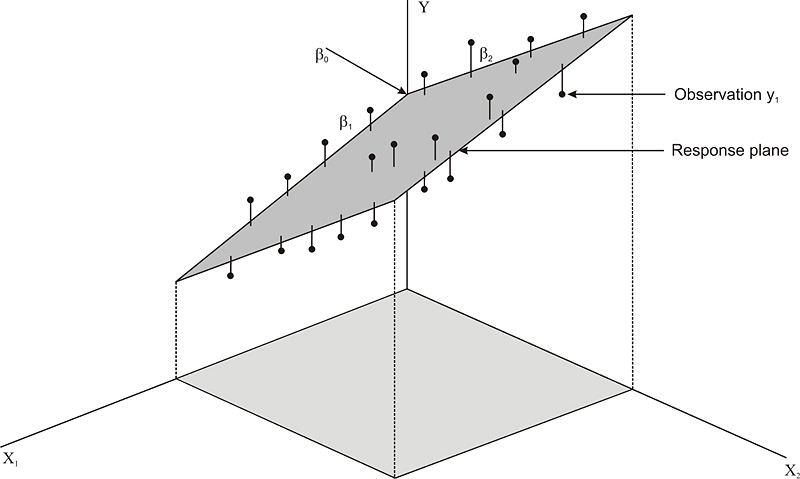
\includegraphics[scale=1.6]{mls}
\end{figure}
}

\frame{\frametitle{Two simple approaches to prediction: }
\framesubtitle{least square for binary response}
\begin{columns}[c]
 \begin{column}{0.5\textwidth}
 \centering
 Simulated data with two variables and two classes: 
$$
Y=\begin{cases}
1&\mbox{orange}\\
0&\mbox{blue}
\end{cases}
$$
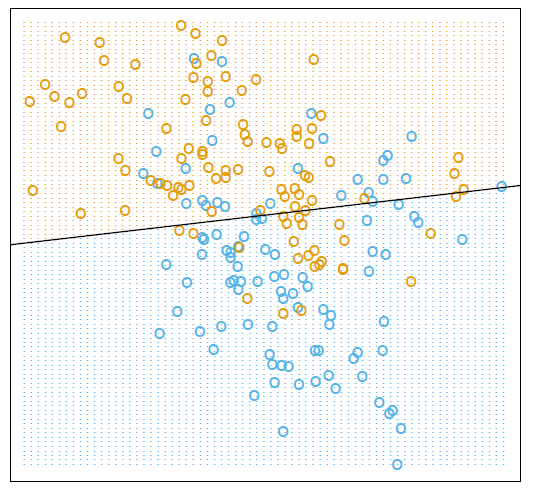
\includegraphics[width=\columnwidth]{LeastSquare.png}
\end{column}
\begin{column}{0.65\textwidth}
If $Y\in\{0,1\}$ is treated \textcolor{uio}{as} a numerical response
$$
\hat Y=\hat\beta_0+\hat\beta_1x_1+\hat\beta_2x_2,
$$
a \textcolor{uio}{prediction rule} 
$$
\hat G=\begin{cases}
1 \mbox{ (orange)}&\mbox{if $\hat Y>0.5$}\\
0 \mbox{ (blue)}&\mbox{otherwise}
\end{cases}
$$
gives linear decision boundary $\{x^T\hat\beta=0.5\}$

\vspace{-0.1cm}

\begin{itemize}
\item optimal under the assumption ``one-Gaussian-per-class'';
\item is it better with nonlinear decision boundary?
\end{itemize}
\end{column}
\end{columns}
}


\frame{\frametitle{Two simple approaches to prediction: }
\framesubtitle{Nearest neighbor methods}
A different approach consists in looking at the \textcolor{uio}{closest} (in the input space) \textcolor{uio}{observations} to $x$ and, based on their output, form $\hat Y(x)$.

\vspace{0.25cm}

The \textcolor{uio}{$k$ nearest neighbors prediction} of $x$ is the mean
$$
\hat{Y}(x)=\frac{1}{k}\sum_{i:x_i\in N_k(x)}y_i,
$$
where \textcolor{uio}{$N_k(x)$} contains the $k$ closest points to $x$.

\begin{itemize}
\item \textcolor{uio}{less assumptions} on $f(x)$;
\item we need to decide $k$;
\item we need to define a metric (for now, consider the Euclidean distance).
\end{itemize}
}


\frame{\frametitle{Two simple approaches to prediction: }
\framesubtitle{nearest neighbor methods}
\begin{columns}
 \begin{column}{0.5\textwidth}
  \centering
Use the same training data (simulated) as before: \hspace{0.6cm}
$$
Y=\begin{cases}
1&\mbox{orange}\\
0&\mbox{blue}
\end{cases}
$$
\vspace{-0.25cm}
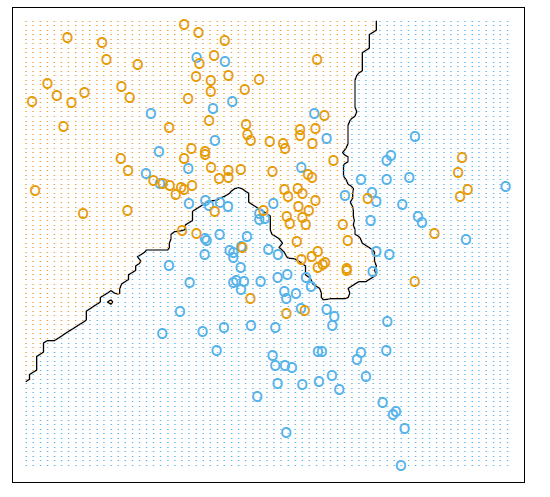
\includegraphics[width=\textwidth]{NearestN.png}
\end{column}
\begin{column}{0.65\textwidth}
\vspace{-1.4cm}

Classify to orange, if there are mostly orange points in the neighborhood: 
$$
\hat G = \begin{cases}
1 \mbox{ (orange)} & \mbox{if } \hat Y>0.5\\
0 \mbox{ (blue)} & \mbox{otherwise}
\end{cases}
$$

\begin{itemize}
\item $k=15$;
\item \textcolor{uio}{flexible} decision boundary;
\item better performance than the linear regression case:
  \begin{itemize}
  \item fewer training observations are missclassified;
  \item is this a good criterion?
  \end{itemize}

\end{itemize}
\end{column}
\end{columns}
}


\frame{\frametitle{Two simple approaches to prediction: }
\framesubtitle{nearest neighbor methods}
\begin{columns}
 \begin{column}{0.5\textwidth}
  \centering
Using the same data as before:
$$
Y=\begin{cases}
1&\mbox{orange}\\
0&\mbox{blue}
\end{cases}
$$

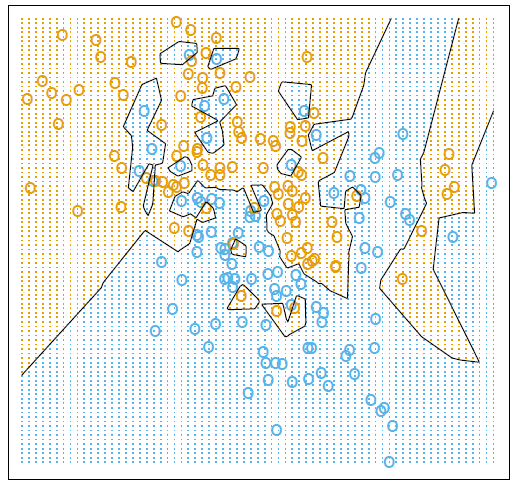
\includegraphics[width=\textwidth]{NearestN2.png}
\end{column}
\begin{column}{0.65\textwidth}
\vspace{-1.15cm}

Note:
\begin{itemize}
\item same approach, with $k=1$;
\item no training observations are missclassified!!!
\item Is this a good solution?
  \begin{itemize}
  \item the learner works greatly on the training set, but what its prediction ability? (remember this term: \textcolor{uio}{overfitting});
  \item It would be preferable to evaluate the performance of the methods in an independent set of observations (\textcolor{uio}{test set});
  \end{itemize}
\item bias-variance trade-off.
\end{itemize}
\end{column}
\end{columns}
}


\frame{\frametitle{Two simple approaches to prediction: }
\framesubtitle{how many neighbors in KNN?}
\centering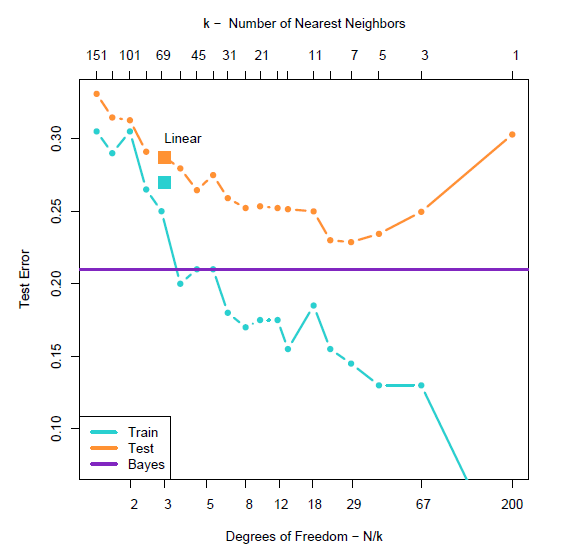
\includegraphics[width=0.7\columnwidth]{Fig24.png}
}


\frame{\frametitle{Two simple approaches to prediction: }
\framesubtitle{alternatives}
Most of the modern techniques are \textcolor{uio}{variants of these two simple procedures}:
\begin{itemize}
\item kernel methods that weight data according to distance;
\item in high dimension: more weight on some variables;
\item local regression models;
\item linear models of functions of $X$;
\item projection pursuit and neural network.
\end{itemize}
}



\subsection{Statistical decision theory}


\frame{\frametitle{Statistical decision theory: }
\framesubtitle{theoretical framework}
\textcolor{uio}{Statistical decision theory} gives a \textcolor{uio}{mathematical framework} for finding the optimal learner.

\vspace{0.5cm}

Let:
\begin{itemize}
  \item $X \in \R^p$ be a p-dimensional random vector of inputs;
  \item $Y \in \R$ be a real value random response variable;
  \item $p(X,Y)$ be their joint distribution;
\end{itemize}

\vspace{0.5cm}

Our goal is to \textcolor{uio}{find} a function \textcolor{uio}{$f(X)$} for \textcolor{uio}{predicting $Y$ given $X$}:
\begin{itemize}
  \item we need a \textcolor{uio}{loss function $L(Y,f(X))$} for \textcolor{uio}{penalizing errors} in $f(X)$ when the truth is $Y$,
  \begin{itemize} 
    \item example: squared error loss, $L(Y,f(X))=(Y-f(X))^2$.
  \end{itemize}
\end{itemize}
}

\frame{\frametitle{Statistical decision theory: }
\framesubtitle{expected prediction error}
Given $p(X,Y)$, it is possible to derive the \textcolor{uio}{expected prediction error} of $f(X)$:
$$
\text{EPE}(f)=E\left[L(Y,f(X))\right]=\int_{x,y}L(y,f(x))p(x,y)dxdy;
$$
we have now a criterion for choosing a learner: find $f$ which \textcolor{uio}{minimizes} $\text{EPE}(f)$.

\vspace{0.5cm}

The aforementioned squared error loss,
$$
L(Y,f(X))=(Y-f(X))^2,
$$
is by far the most common and convenient loss function. Let us focus on it!
}


\frame{\frametitle{Statistical decision theory: }
\framesubtitle{squared error loss}
If $L(Y,f(X))=(Y-f(X))^2$, then
\begin{align*}
\text{EPE}(f)
=&E_{X,Y}[(Y-f(X))^2]\\
=&E_{X}E_{Y|X}[(Y-f(X))^2|X]
\end{align*}

It is then sufficient to \textcolor{uio}{minimize} $E_{Y|X}[(Y-f(X))^2|X]$ for each $X$:
$$
f(x)=\text{argmin}_cE_{Y|X}[(Y-c)^2|X=x],
$$ 
which leads to
$$
f(x)=E[Y|X=x],
$$
i.e., the \textcolor{uio}{conditional expectation}, also known as \textcolor{uio}{regression function}.

\vspace{0.5cm}

Thus, by average squared error, the \textcolor{uio}{best prediction of $Y$} at any point $X=x$ is the \textcolor{uio}{conditional mean}.
}


\frame{\frametitle{Statistical decision theory: }
\framesubtitle{estimation of optimal $f$}
In practice, \textcolor{uio}{$f(x)$ must be estimated}.

\vspace{0.25cm}

{\bf \underline{Linear regression:}}
\begin{itemize}
  \item \textcolor{uio}{assumes a function} linear in its arguments, $f(x)\approx x^T\beta$;
  \item $\text{argmin}_\beta E[(Y-X^T\beta)^2] \rightarrow \beta=E[XX^T]^{-1}E[XY]$;
  \item replacing the expectations by averages over the training data leads to $\hat{\beta}$.
  \item Note:
  \begin{itemize}
	\item no conditioning on $X$;
	\item we have used our knowledge on the functional relationship to pool over all values of $X$ (model-based approach);
	\item less rigid functional relationship may be considered, e.g.
	$$
	f(x)\approx \sum_{j=1}^p f_j(x_j).
	$$
  \end{itemize}
\end{itemize}
}


\frame{\frametitle{Statistical decision theory: }
\framesubtitle{estimation of optimal $f$}
{\bf \underline{$K$ nearest neighbors:}}
\begin{itemize}
  \item uses \textcolor{uio}{directly} $f(x)=E[Y|X=x]$:
  \item $\hat f(x_i)= \text{Ave}(y_i)$ for observed $x_i$'s;
  \item normally there is \textcolor{uio}{at most} one observation for each point $x_i$;
  \item uses points in the \textcolor{uio}{neighborhood},
  $$
  \hat f(x)=\text{Ave}(y_i|x_i\in N_k(x))
  $$
  \item there are two approximations:
  \begin{itemize}
    \item \textcolor{uio}{expectation} is approximated by \textcolor{uio}{averaging} over sample data;
    \item conditioning on a \textcolor{uio}{point} is relaxed to conditioning on a \textcolor{uio}{neighborhood}.
  \end{itemize}
\end{itemize}
}


\frame{\frametitle{Statistical decision theory: }
\framesubtitle{estimation of optimal $f$}
\begin{itemize}
  \item assumption of $k$ nearest neighbors: $f(x)$ can be approximated by a \textcolor{uio}{locally constant function};
  \item for $N \rightarrow \infty$, all $x_i\in N_k(x) \approx x$;
  \item for $k \rightarrow \infty$, $\hat f(x)$ is getting more stable;
  \item under mild regularity condition on $p(X,Y)$,
  $$
  \textcolor{uio}{\hat{f}(x) \rightarrow E[Y|X = x] \text{ for } N,k \rightarrow \infty \text{ s.t. } k/N \rightarrow 0}
  $$
  \item is this an universal solution?
  \begin{itemize}
    \item small sample size;
    \item curse of dimensionality (see later)
  \end{itemize}
\end{itemize}
}


\frame{\frametitle{Statistical decision theory: }
\framesubtitle{other loss function}
\begin{itemize}
  \item It is \textcolor{uio}{not necessary} to implement the squared error loss function ($L_2$ loss function);
  \item a \textcolor{uio}{valid alternative} is the \textcolor{uio}{$L_1$ loss function}:
  \begin{itemize}
  	\item the solution is the \textcolor{uio}{conditional median}
    $$
    \hat f(x)=\text{median}(Y|X=x)
    $$
    \item \textcolor{uio}{more robust estimates} than those obtained with the conditional mean;
    \item the $L_1$ loss function has \textcolor{uio}{discontinuities in its derivatives} $\rightarrow$ numerical difficulties.
  \end{itemize}
\end{itemize}
}


\frame{\frametitle{Statistical decision theory: }
\framesubtitle{other loss functions}
What happens with a \textcolor{uio}{categorical outcome} $G$?
\begin{itemize}
  \item similar concept, different loss function;
  \item $G \in \mathcal{G}=\{1,\dots,K\} \rightarrow \hat{G} \in \mathcal{G}=\{1,\dots,K\}$;
  \item $L(G,\hat{G})=L_{G,\hat{G}}$ a \textcolor{uio}{$K\times K$ matrix}, where $K=|G|$;
  \item each element of the matrix $l_{ij}$ is the \textcolor{uio}{price to pay to missallocate} category $g_i$ as $g_j$
  \begin{itemize}
    \item all elements on the diagonal are 0;
    \item often non-diagonal elements are 1 (zero-one loss function).
  \end{itemize}
\end{itemize}
}


\frame{\frametitle{Statistical decision theory: }
\framesubtitle{other loss functions}
Mathematically:

\vspace{-0.5cm}

{\small
\begin{align*}
EPE =& E_{G,X}[L(G,\hat{G}(X))] \\
	=& E_X\left[E_{G|X}[L(G,\hat{G}(X))]\right] \\
	=& E_X\left[ \sum_{k=1}^K L(g_k,\hat{G}(X))\P(G=g_k|X=x) \right]\\
\end{align*}
}

\vspace{-1cm}

which is sufficient to be minimized pointwise, i.e,
{\small
\setlength{\belowdisplayskip}{1pt}\setlength{\abovedisplayskip}{1pt}
$$
\hat{G}=\text{argmin}_{g\in\mathcal{G}} \sum_{k=1}^K L(g_k,g)\P(G=g_k|X=x).
$$
}
When using the 0-1 loss function
{\small
\setlength{\abovedisplayskip}{2pt}
\begin{align*}
\hat{G} =&\text{argmin}_{g\in\mathcal{G}} \sum_{k=1}^K \{1-\mathds{1}(G=g_k))\}\P(G=g_k|X=x)\\
        =&\text{argmin}_{g\in\mathcal{G}} \{1-\P(G=g_k|X=x)\}\\
        =&\text{argmax}_{g\in\mathcal{G}} \P(G=g_k|X=x)\\
\end{align*}
}
}



\frame{\frametitle{Statistical decision theory: }
\framesubtitle{other loss functions}
Alternatively,
$$
\hat{G}(x)= g_k \mbox{  if  } P(G=g_k|X=x) = \max_{g\in \mathcal{G}}\Pr(G=g|X=x),
$$
also known as \textcolor{uio}{Bayes classifier}.

\begin{columns}[c]
\begin{column}{0.5\textwidth}
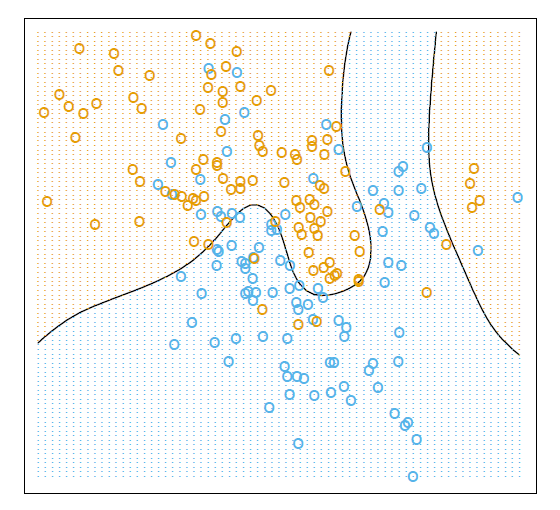
\includegraphics[width=1\columnwidth]{Bayes.png}
\end{column}
\begin{column}{0.65\textwidth}

\begin{itemize}
  \item $k$ nearest neighbor: 
  \begin{itemize}
    \item $\hat{G}(x)=$ category with largest frequency in $k$ nearest samples;
    \item approximation of this solution.
  \end{itemize}
  \item regression:
  \begin{itemize}
    \item $E[Y_k|X]=\P(G=g_k|X)$;
    \item also approximates the Bayes classifier.
  \end{itemize}
  
  \end{itemize}
\end{column}
\end{columns}
}


\subsection{Local methods in high dimensions}


\frame{\frametitle{Local methods in high dimensions}
The two (extreme) methods seen so far:
\begin{itemize}
\item linear model, \textcolor{uio}{stable but biased};
\item $k$-nearest neighbor, \textcolor{uio}{less biased but less stable}.
\end{itemize}

\vspace{0.5cm}

For large set of training data:
\begin{itemize}
\item always possible to use $k$ nearest neighbors?
\item Breaks down in high dimensions $\rightarrow$ \textcolor{uio}{curse of dimensionality} \citep{Bellman1961}.
\end{itemize}
}


\frame{\frametitle{Local methods in high dimensions: }
\framesubtitle{curse of dimensionality}
\begin{columns}[c]
\begin{column}{0.4\textwidth}
  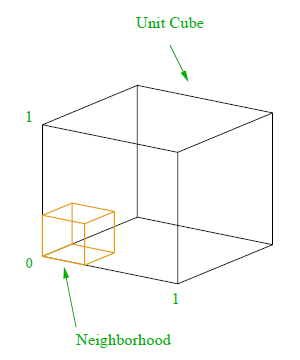
\includegraphics[width=\textwidth]{Fig26a.png}
\end{column}
\begin{column}{0.6\textwidth}
\begin{itemize}
\item Assume $X\sim\text{Unif}[0,1]^p$;
\item define $e_p$ the \textcolor{uio}{expected length size} of a hypercube containing a fraction $r$ of input points;
\item $e_p(r)=r^{1/p}$ ($e^p=r \Leftrightarrow e=r^{1/p}$);
\end{itemize}
\end{column}
\end{columns}
}


\frame{\frametitle{Local methods in high dimensions: }
\framesubtitle{curse of dimensionality}
\begin{columns}[c]
\hspace{-1cm}
\begin{column}{0.4\textwidth}
  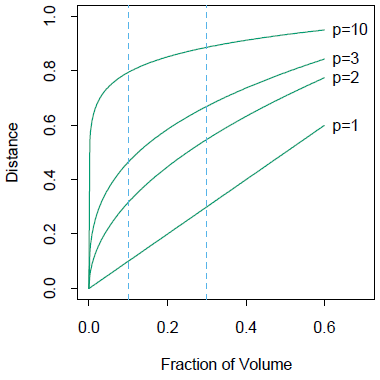
\includegraphics[width=1.25\textwidth]{Fig26b.png}
\end{column}
\begin{column}{0.6\textwidth}
\begin{itemize}
\item Expected length: $e_p(r)=r^{1/p}$ 
{
\begin{tabular}{crrrr}
\hline
$p$        &1&2&3&5\\
\hline
$e_p(0.01)$&0.01& 0.10& 0.22& 0.63\\
$e_p(0.1)$ &0.10& 0.32& 0.46& 0.79\\
\hline
\end{tabular}
}
\end{itemize}
\end{column}
\end{columns}
}


\frame{\frametitle{Local methods in high dimensions: }
\framesubtitle{curse of dimensionality}
\begin{columns}[c]
\begin{column}{0.5\textwidth}
Assume $Y=f(X)=e^{-8||X||^2}$

\vspace{0.25cm}

and use the 1-nearest neighbor to predict $y_0$ at $x_0=0$, i.e.

\vspace{0.25cm}

$\hat y_0= y_i \mbox{ s.t. } x_i \text{ nearest observed}$  \\\vspace{0.5\baselineskip}

\vspace{-0.5cm}

{\small
\begin{align*}
\text{MSE}&(x_0) = \\
=&E_{\cal T}[\hat y_0-f(x_0)]^2  \\
=&E_{\cal T}[\hat y_0-E_{\cal T}(\hat y_0)]^2 \\
&\quad+ [E_{\cal T}(\hat y_0)-f(x_0)]^2\\
=&\text{Var}(\hat y_0)+\text{Bias}^2(\hat y_0)&
\end{align*}
}

\vspace{-0.5cm}

NB: we will see often this bias-variance decomposition!
\end{column}
\begin{column}{0.6\textwidth}
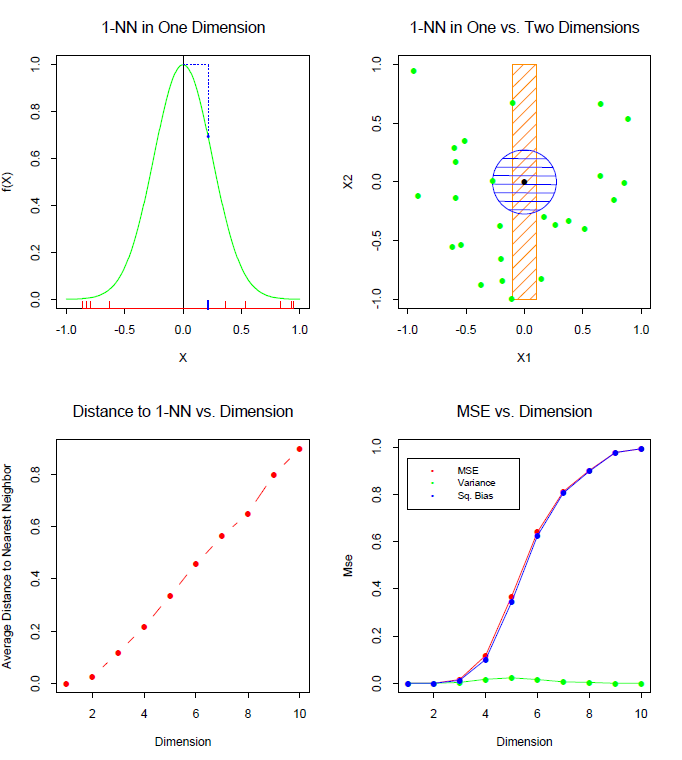
\includegraphics[width=\columnwidth]{Fig27.png}
\end{column}
\end{columns}
}


\frame{\frametitle{Local methods in high dimensions: }
\framesubtitle{EPE in the linear model}
\begin{itemize}
\item Assume now $Y=X^T\beta+\varepsilon$
\item we want to predict $y_0=x_0^T\beta+\varepsilon_0$ with $x_0$ fixed
\item $\hat y_0=x_0^T\hat\beta$ where $\hat\beta=(X^T X)^{-1} X^T y$
\end{itemize}\begin{align*}
\text{EPE}&(x_0)=E(y_0-\hat y_0)^2\\
=&E\left[\left(y_0-E[y_0|x_0]+E[y_0|x_0]-E[\hat y_0|x_0]+E[\hat y_0|x_0]-\hat y_0\right)^2\right]\\
=&E(y_0-E[y_0|x_0])^2+(E[y_0|x_0]-E[\hat y_0|x_0])^2 \\
\qquad &+E(\hat y_0- E[\hat y_0|x_0])^2\\ 
=&\text{Var}(y_0|x_0)+\text{Bias}^2(\hat y_0)+\text{Var}(\hat y_0)
\end{align*} 

True and assumed linear model
\begin{itemize}
\item Bias=0
\item $\text{Var}(\hat y_0)=x_0^TE(X^TX)^{-1}x_0\sigma^2$
\item $\text{EPE}(x_0)=\sigma^2+x_0^TE(X^TX)^{-1}x_0\sigma^2$
\end{itemize}
}


\frame{\frametitle{Local methods in high dimensions: }
\framesubtitle{EPE in the linear model}
\begin{itemize}
\item $\text{EPE}(x_0)=\sigma^2+x_0^TE(X^TX)^{-1}x_0\sigma^2$
\item If $x$'s drawn from a random distribution with $E(X)=0$, $X^TX\rightarrow N\text{Cov}(X)$
\item Assume also $x_0$ drawn from same distribution:
\begin{align*}
E_{x_0}\left[\text{EPE}(x_0)\right] \approx& \sigma^2+E_{x_0}[x_0^T\text{Cov}(X)^{-1}x_0]N^{-1}\sigma^2\\
=&\sigma^2+N^{-1}\sigma^2\text{trace}[\text{Cov}(X)^{-1}E_{x_0}[x_0x_0^T]]\\
=&\sigma^2+N^{-1}\sigma^2\text{trace}[\text{Cov}(X)^{-1}\text{Cov}(x_0)]\\
=&\sigma^2+N^{-1}\sigma^2\text{trace}[I_p]\\
=&\sigma^2+N^{-1}\sigma^2p
\end{align*}
\item It increases linearly with $p$!
\end{itemize}
}



\subsection{Data science, statistics, machine learning}


\frame{\frametitle{Data science, statistics, machine learning: }
\framesubtitle{what is ``data science''?}

\cite{CarmichaelMarron2018} stated: ``Data science is the business of \textcolor{uio}{learning from data}'', immediately followed by ``which is traditionally the business of statistics''.

\hspace{2pt}

What is your opinion?
\begin{itemize}
\item ``\emph{data science} is simply a \textcolor{uio}{rebranding} of \emph{statistics}'' \\
\citep[``data science is statistics on a Mac'',][]{Bhardwaj2017}
\item ``\emph{data science} is a \textcolor{uio}{subset} of \emph{statistics}'' \\
\citep[``a \emph{data scientist} is a statistician who lives in San Francisco'',][]{Bhardwaj2017}
\item ``\emph{statistics} is a \textcolor{uio}{subset} of \emph{data scientist}'' \\
\citep[``statistics is the least important part of data science'',][]{Gelman2013}
\end{itemize}
}


\frame{\frametitle{Data science, statistics, machine learning: }
\framesubtitle{what is ``data science''?}
\centering
\begin{figure}
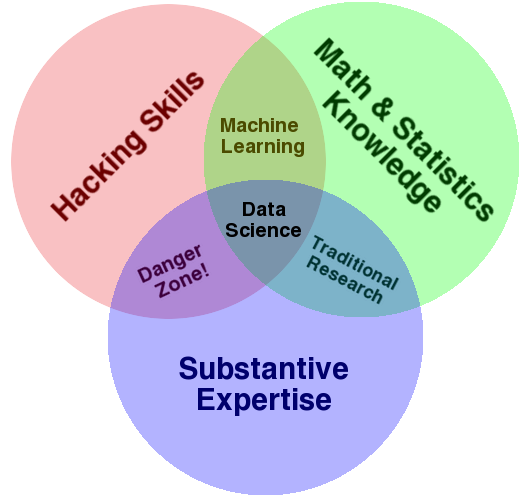
\includegraphics[width=0.72\textwidth]{Data_Science_VD}
\end{figure}
}


\frame{\frametitle{Data science, statistics, machine learning: }
\framesubtitle{statistics vs machine learning}
What about differences between \textcolor{uio}{statistics} and \textcolor{uio}{machine learning}?
\begin{itemize}
\item[]
\item ``Machine learning is essentially a form of applied statistics'';
\item ``Machine learning is glorified statistics'';
\item ``Machine learning is statistics scaled up to big data'';
\item ``The short answer is that there is no difference'';
\item[]
\end{itemize}

(\url{https://www.svds.com/machine-learning-vs-statistics})
}



\frame{\frametitle{Data science, statistics, machine learning: }
\framesubtitle{statistics vs machine learning}
Let us be a little bit more provocative \dots
\begin{itemize}
\item[]
\item ``Machine learning is for Computer Science majors who couldn't pass a Statistics course'';
\item ``Machine learning is Statistics minus any checking of models and assumptions'';
\item ``I don't know what Machine Learning will look like in ten years, but whatever it is I'm sure Statisticians will be whining that they did it earlier and better''.
\item[]
\end{itemize}

(\url{https://www.svds.com/machine-learning-vs-statistics})
}

\frame{\frametitle{Data science, statistics, machine learning: }
\framesubtitle{statistics vs machine learning}
``The difference, as we see it, is not one of algorithms or practices but of \textcolor{uio}{\emph{goals} and \emph{strategies}}. 

\textcolor{uio}{Neither field is a subset of the other}, and neither lays exclusive claim to a technique. They are like two pairs of old men sitting in a park playing two different board games. Both games use the same type of board and the same set of pieces, but \textcolor{uio}{each plays by different rules and has a different goal} because the games are fundamentally different. Each pair looks at the other's board with bemusement and thinks they're not very good at the game.''

\hspace{2pt}

``Both Statistics and Machine Learning create models from data, but for \textcolor{uio}{different purposes}.''

\hspace{2pt}

(\url{https://www.svds.com/machine-learning-vs-statistics})
}

\frame{\frametitle{Data science, statistics, machine learning: }
\framesubtitle{statistics vs machine learning}

\underline{\bf Statistics}

\begin{itemize}

\item ``The goal of modeling is approximating and then understanding the \textcolor{uio}{data-generating process}, with the goal of answering the question you actually care about.''

\item ``The models provide the \textcolor{uio}{mathematical framework} needed to make \textcolor{uio}{estimations and predictions}.''

\item ``The goal is to prepare every statistical analysis as if you were going to be an expert witness at a trial. [\dots] \textcolor{uio}{each choice made in the analysis must be defensible}.''

\item ``\textcolor{uio}{The analysis is the final product}. Ideally, every step should be documented and supported, [\dots] each assumption of the model should be listed and checked, every diagnostic test run and its results reported.''

\end{itemize}

(\url{https://www.svds.com/machine-learning-vs-statistics})
}


\frame{\frametitle{Data science, statistics, machine learning: }
\framesubtitle{statistics vs machine learning}

\underline{\bf Statistics}

\begin{itemize}
\item ``In conclusion, the Statistician is concerned primarily with \textcolor{uio}{model validity}, \textcolor{uio}{accurate estimation} of model parameters, and \textcolor{uio}{inference} from the model. However, prediction of unseen data points, a major concern of Machine Learning, is less of a concern to the statistician. Statisticians have the techniques to do \textcolor{uio}{prediction}, but these are \textcolor{uio}{just special cases of inference} in general.''
\end{itemize}

(\url{https://www.svds.com/machine-learning-vs-statistics})
}

\frame{\frametitle{Data science, statistics, machine learning: }
\framesubtitle{statistics vs machine learning}

\underline{\bf Machine Learning}

\begin{itemize}

\item ``The \textcolor{uio}{predominant task is predictive} modeling''

\item ``The model does not represent a belief about or a commitment to the data generation process. [\dots] \textcolor{uio}{the model is really only instrumental to its performance}.''

\item ``The proof of the model is in the \textcolor{uio}{test set}.''

  \item ``\textcolor{uio}{freed from worrying about model assumptions or diagnostics}. [\dots] are only a problem if they cause bad predictions.''
  \item ``\textcolor{uio}{freed from worrying} about difficult cases \textcolor{uio}{where assumptions are violated}, yet the model may work anyway.''
  \item ``The samples are chosen [\dots] from a static population, and are representative of that population. \textcolor{uio}{If the population changes} [\dots] \textcolor{uio}{all bets are off}.''

\end{itemize}

(\url{https://www.svds.com/machine-learning-vs-statistics})
}



\frame{\frametitle{Data science, statistics, machine learning: }
\framesubtitle{statistics vs machine learning}

\underline{\bf Machine Learning}

\begin{itemize}

\item ``Because ML practitioners do not have to justify model choice or test assumptions, they are free to choose from among a \textcolor{uio}{much larger set of models}. In essence, all ML techniques employ \textcolor{uio}{a single diagnostic test: the prediction performance} on a holdout set.''

\item ``As a typical example, consider random forests and boosted decision trees. The theory of how these work is well known and understood. [\dots] Neither has diagnostic tests nor assumptions about when they can and cannot be used. Both are \textcolor{uio}{``black box'' models} that produce nearly \textcolor{uio}{unintelligible classifiers}. For these reasons, a Statistician would be reluctant to choose them. Yet they are \textcolor{uio}{surprisingly -- almost amazingly -- successful at prediction problems}.''

\end{itemize}

(\url{https://www.svds.com/machine-learning-vs-statistics})
}


\frame{\frametitle{Data science, statistics, machine learning: }
\framesubtitle{statistics vs machine learning}

\underline{\bf Machine Learning}

\begin{itemize}

\item ``In summary, \textcolor{uio}{both Statistics and Machine Learning contribute to Data Science} but they have different goals and make different contributions. Though the methods and reasoning may overlap, the purposes rarely do. Calling Machine Learning “applied Statistics” is misleading, and does a disservice to both fields.''

\item ``Computer scientists are taught to design real-world algorithms that will be used as part of software packages, while statisticians are trained to provide the mathematical foundation for scientific research. [\dots] Putting the two groups \textcolor{uio}{together into a common data science team} (while often adding individuals trained in other scientific fields) can create a \textcolor{uio}{very interesting} team dynamic.''
\end{itemize}

(\url{https://www.svds.com/machine-learning-vs-statistics})
}



%%%%%%%%%%%
\section*{Bibliography}
%%%%%%%%%%%

\frame[allowframebreaks]{\frametitle{References}
\footnotesize
\bibliographystyle{../../../../support/biometrika}
\bibliography{../../../../support/biblio}
}

\end{document}
